\documentclass{article}

\usepackage[english, russian]{babel}
\usepackage{amsmath}
\newcommand{\Mod}[1]{\ (\mathrm{mod}\ #1)}
\usepackage[letterpaper,top=2cm,bottom=2cm,left=3cm,right=3cm,marginparwidth=1.75cm]{geometry}
\usepackage[usenames,dvipsnames]{color}

\setlength{\abovedisplayskip}{3pt}
\setlength{\abovedisplayshortskip}{3pt}
\setlength{\belowdisplayskip}{3pt}
\setlength{\belowdisplayshortskip}{3pt}
\usepackage[14pt]{extsizes} 

\DeclareMathAlphabet{\pazocal}{OMS}{zplm}{m}{n}
\newcommand{\unif}{\pazocal{U}}

\linespread{1.6}

\usepackage{amsmath}
\usepackage{graphicx}
\usepackage[colorlinks=true, allcolors=blue]{hyperref}
\usepackage{fancyvrb} % for "\Verb" macro
\VerbatimFootnotes    % enable use of \Verb in footnotes

\title{Интрукция по запуску}
\date{}
\begin{document}
\maketitle

\section*{Необходимые зависимости}

\begin{itemize}
\item {Для работы модели ЦОД необходим EnergyPlus версии 23.1.0, скачать можно с официального сайта \href{https://energyplus.net/downloads}{здесь}. Путь до скрипта EnergyPlus можно специфицировать в \Verb+config.py+}

\item{Python версии 3.9.16 (или любой другой совместимой с этой версией), а также зависимости указанные в \Verb+requirements.txt+.}

\item {Запущенные контейнеры с ClickHouse и Superset. По умолчанию проект настроен на конфиги как в \href{https://github.com/YARIK-AI/ML}{YARIK-AI}. Оттуда нужны контейнеры clickhouse, postgres-superset и superset.}

\item{Для просмотра статистик необходим JupyterNotebook, поставить его можно или отдельно или как контейнер jupyter в \href{https://github.com/YARIK-AI/ML}{YARIK-AI}.}

\item{Для более удобного запуска комманд подойдет утилита make}

\\
Проверить корректен ли путь до EnergyPlus и стоит ли нужная версия Python можно запустив:\\
\Verb+ make test_env+ (или \Verb+python test_environment.py+). 
\end{itemize}

\section*{Основные команды}
Для просмотра полного списка команд с их кратким описанием можно написать \Verb+make help+. 

\section*{Пример работы}
Сделаем симуляцию инференса модели.

Запустим http-API для RL-агента:\\
\Verb+make raise_server+ (или \Verb+python main.py raise_server+)

Теперь, когда сервер запущен, можно запуcтить симуляцию:\\ 
\Verb+make simulate_inference+ (или \Verb+python main.py simulate_inference+)

Пойдет процесс симуляции, создасться БД и таблица в ClickHouse, туда будут записываться логи от модели ЦОД.

Посмотрим, какие данные загрузились зайдя по хосту кликхауса и выпонлив select-запрос (Рис. \ref{fig:CH-select}).

\begin{figure}[h]

\centering

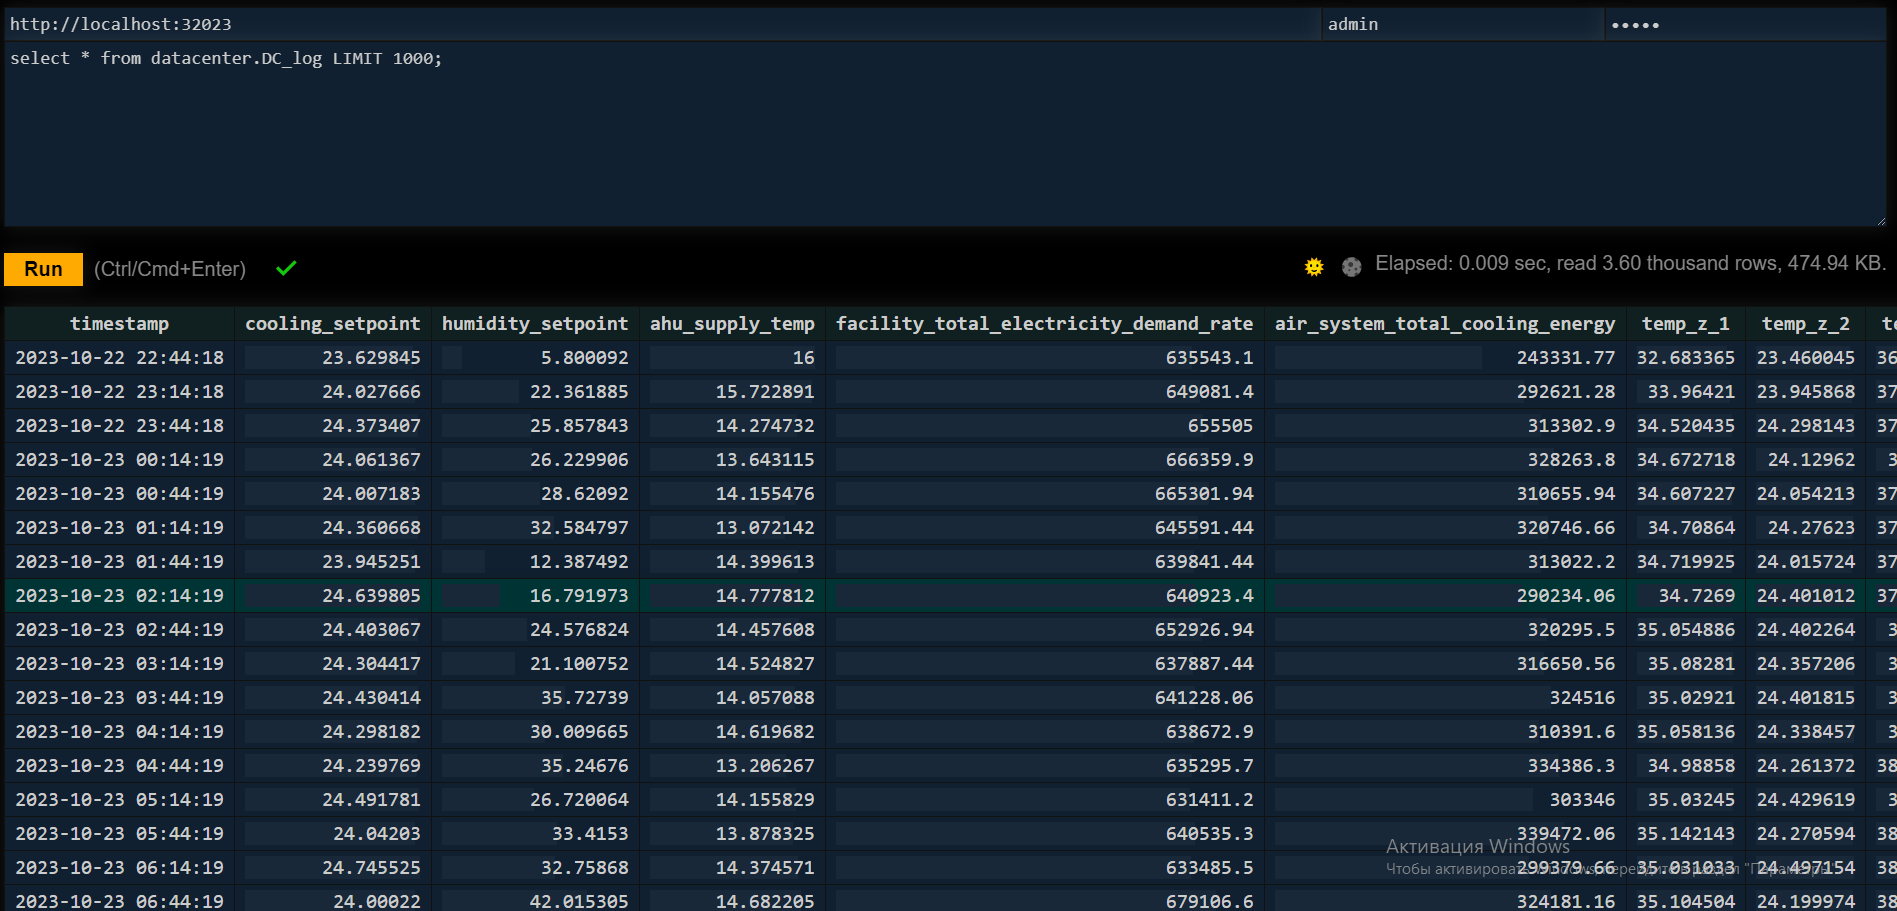
\includegraphics[width=0.95\linewidth]{figures/clickhouse_select.png}

\caption{Пример выборки данных из созданной таблицы в ClickHouse.}

\label{fig:CH-select}

\end{figure}
Далее зайдем в Superset и импортируем дэшборд, который находится в \Verb+external/DC_dashboard.zip+. Это автоматически подгрузит данные из нужной таблицы ClickHouse, графики и сам дэшборд (Рис. \ref{fig:superset-dashboard}).

\begin{figure}[h]

\centering

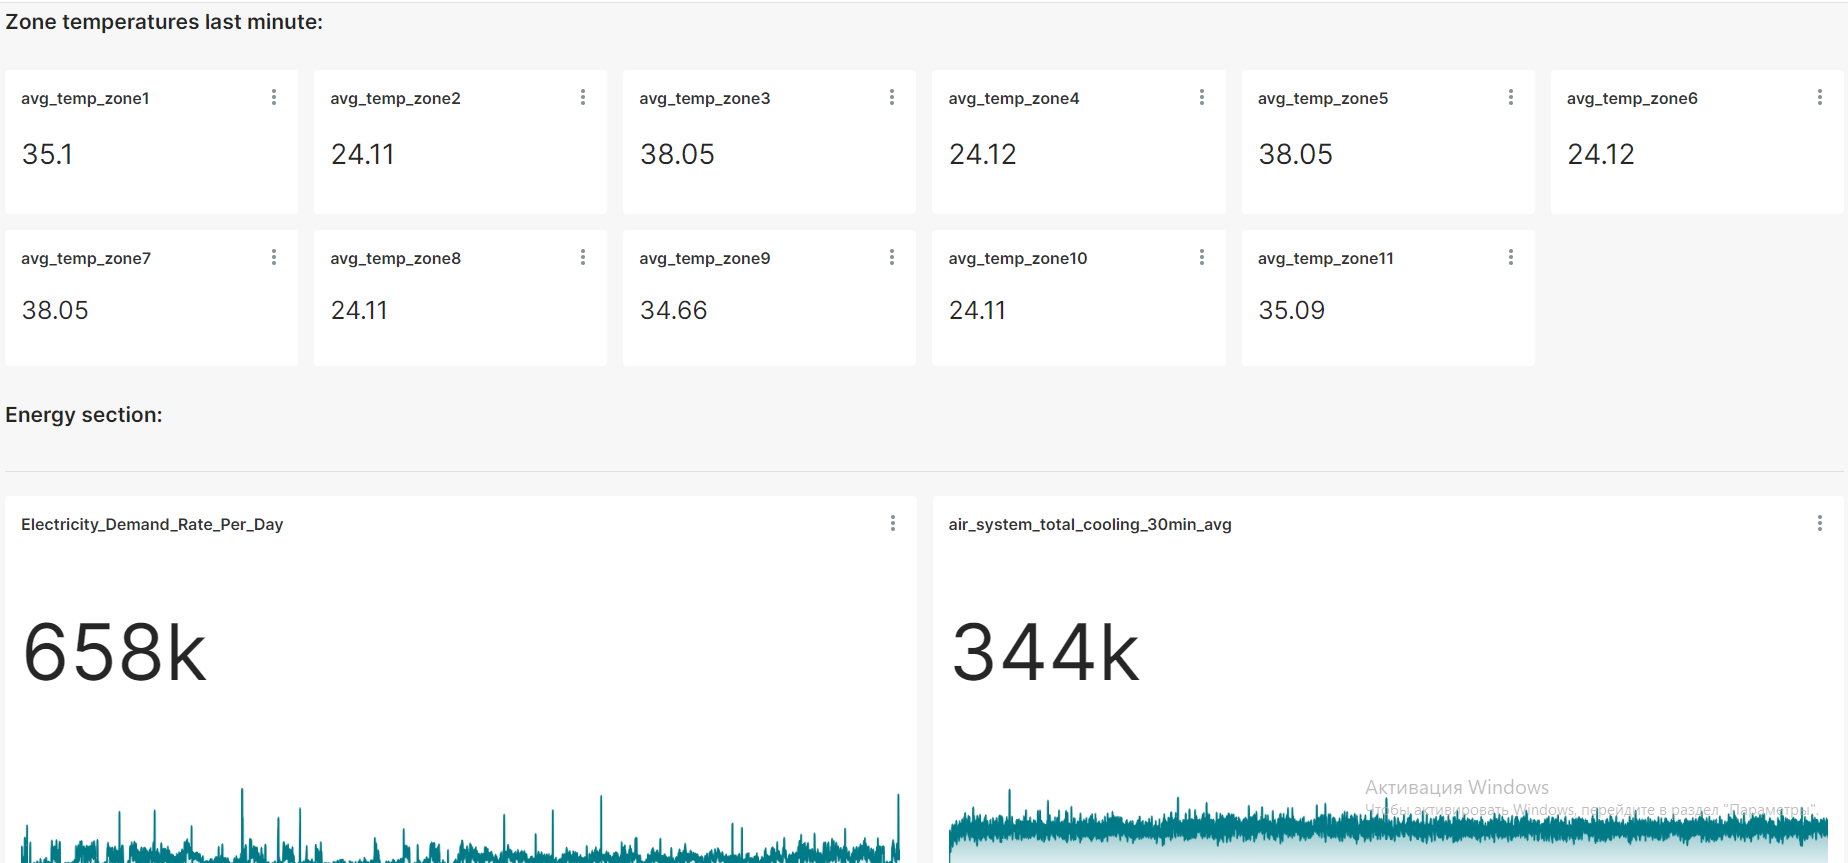
\includegraphics[width=0.95\linewidth]{figures/Superset_dashboard.png}

\caption{Часть дэшборда для ЦОД в Superset.}

\label{fig:superset-dashboard}

\end{figure}


\end{document}